\section{Evaluation of the model}
\comm{Main content:
- Are the estimates by the authors realistic?
- reliability: would we be able to replicate the model with newer data? Would the construction of the model still work or is it a one-time-only model that only works with the data from 2009?
- what to enhance in the paper?
- convergence of the model? what do the plots say?}
The model involves a number of short-comings regarding its notation and mathematical formulation, and many errors have been reported above. In general, following the verified approach by Rossi et al. should ensure a conclusive model. From a mathematical perspective, the chosen levels of hierarchy, the way to account for endogeneity and the chosen logit function make sense despite the level of complexity. The simultaneity however adds a certain fragility to the method, the numbers, and thus the reliability of the instrument as a whole. This system cannot be easily reproduced nor can the correctness of the results be cross-validated.\\
Furthermore, some parameters, such as data on competitors, are completely missing. This forced us to focus on each particular detail of the model and effectively interpret the missing data in the most probable way according to our interpretation. While this is the only approach we could have taken given the scarcity of the data, it made us question the accurateness of the estimations and whether the results can still hold.\\
Another thing worth mentioning is that the model described in the paper cannot be replicated entirely due to a different layout of Google search pages. The positioning of both organic and paid ads has changed a great deal since 2009 (when the experiment in the Agarwal et al. paper was conducted), which also means that the way users interact with the ads would not be the same today. Examples of ad positions then and now are provided below: Figure \ref{fig:Google2009} from 2009 is taken from the paper itself, while the current one in Figure \ref{fig:Googletoday} is prepared by the group.\\

\begin{figure}
    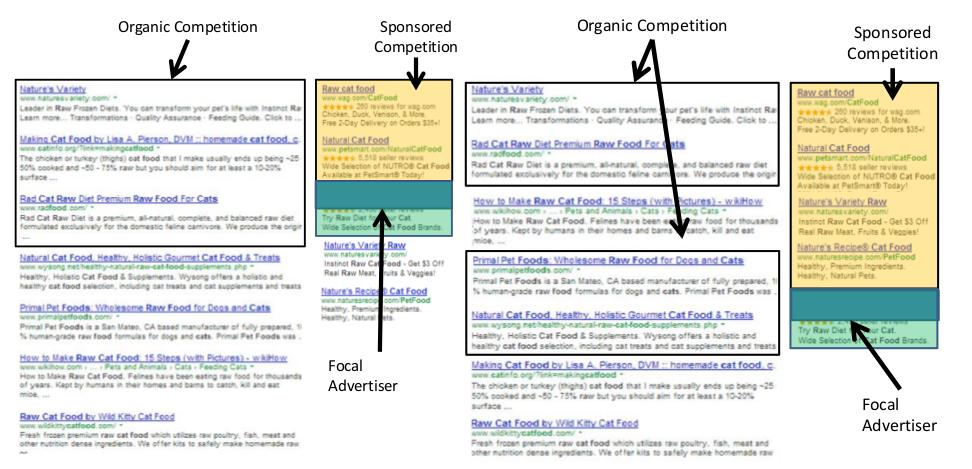
\includegraphics[scale=0.35]{organic_vs_sponsored.jpeg}
    \caption{Google ad positions in 2009}
    \label{fig:Google2009}
\end{figure}

\begin{figure}
    \centering
    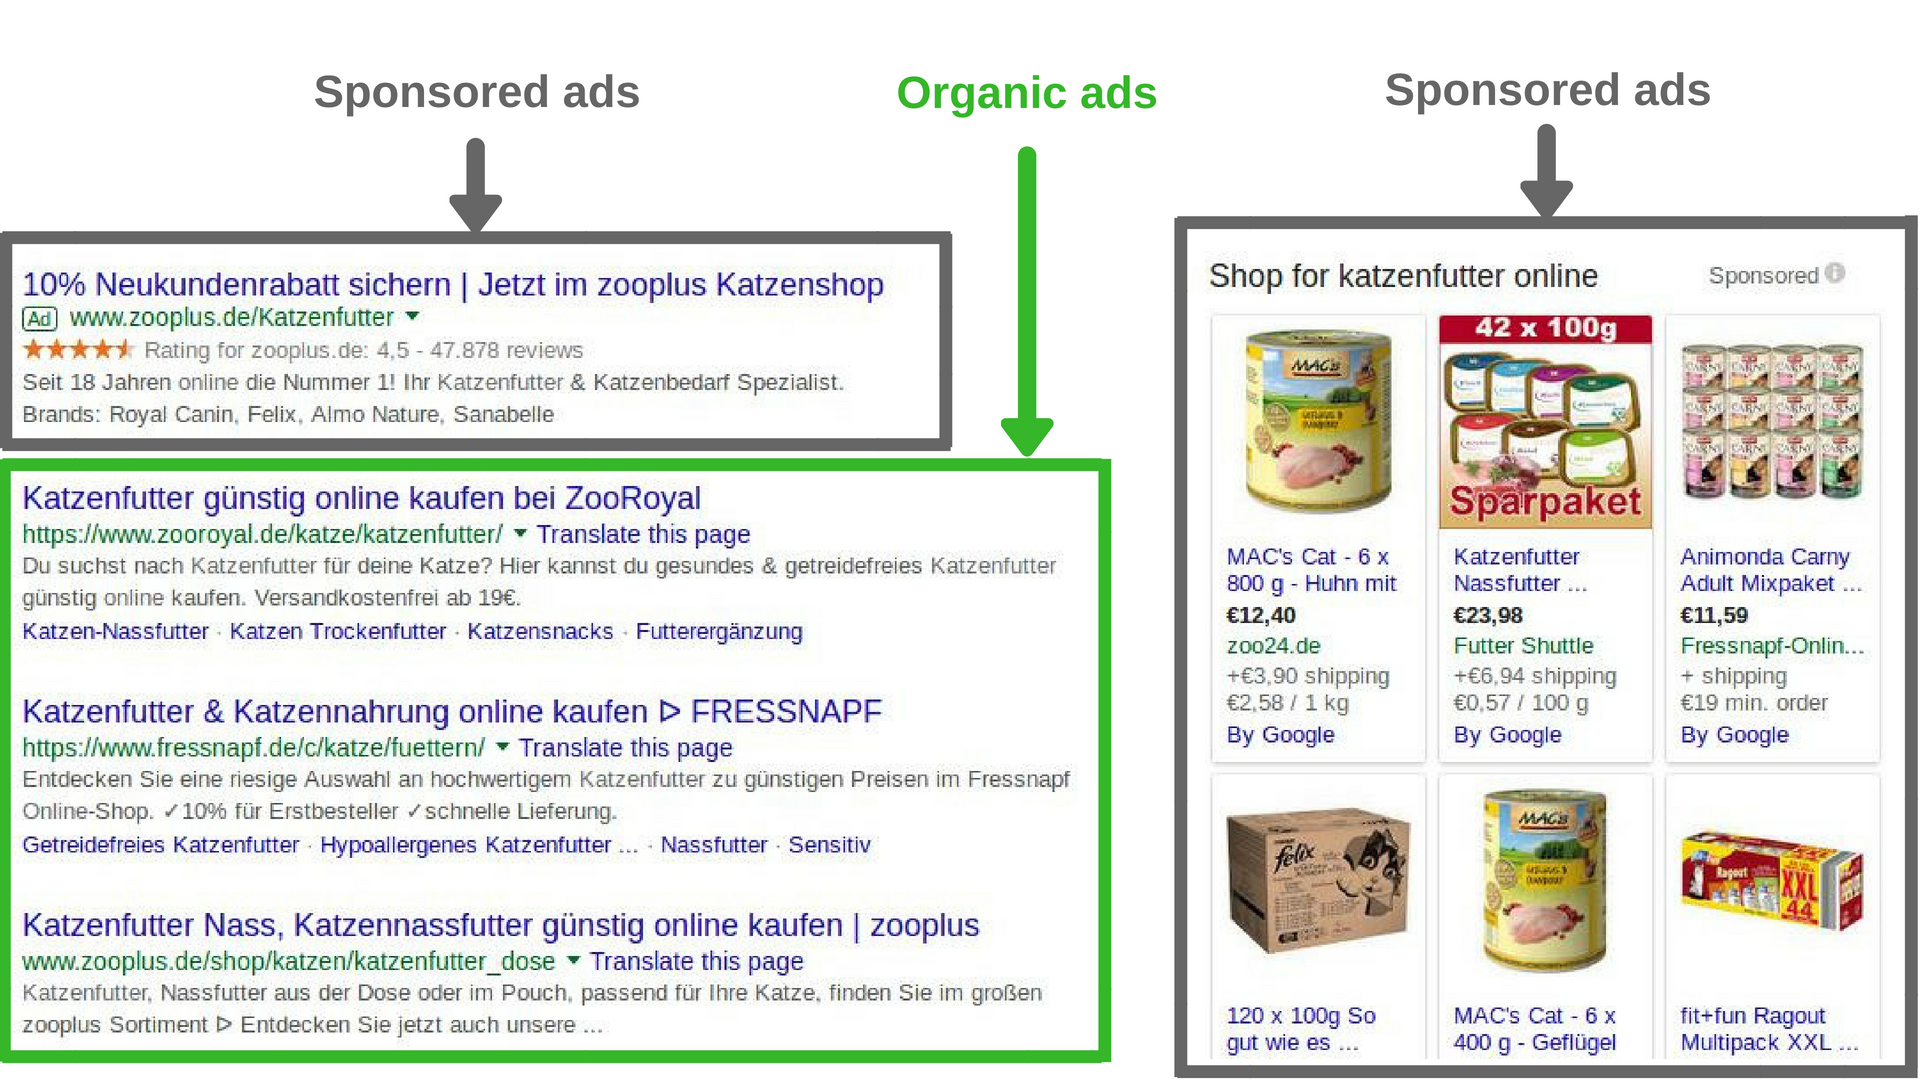
\includegraphics[scale=0.2]{catfoodsearch.png} 
    \caption{Google ad positions today}
    \label{fig:Googletoday}
\end{figure}

\newpage
All in all, the model by Agarwal et al. posed quite a few challenges when trying to follow the approach. The model as such, and especially its documentation, could be improved in the future. We would like to close this paper with a small statement: if pet food were a problem, then the most simple solution might be the correct one, according to William of Ockham. Just give the dogs some petfood.

\begin{center}
    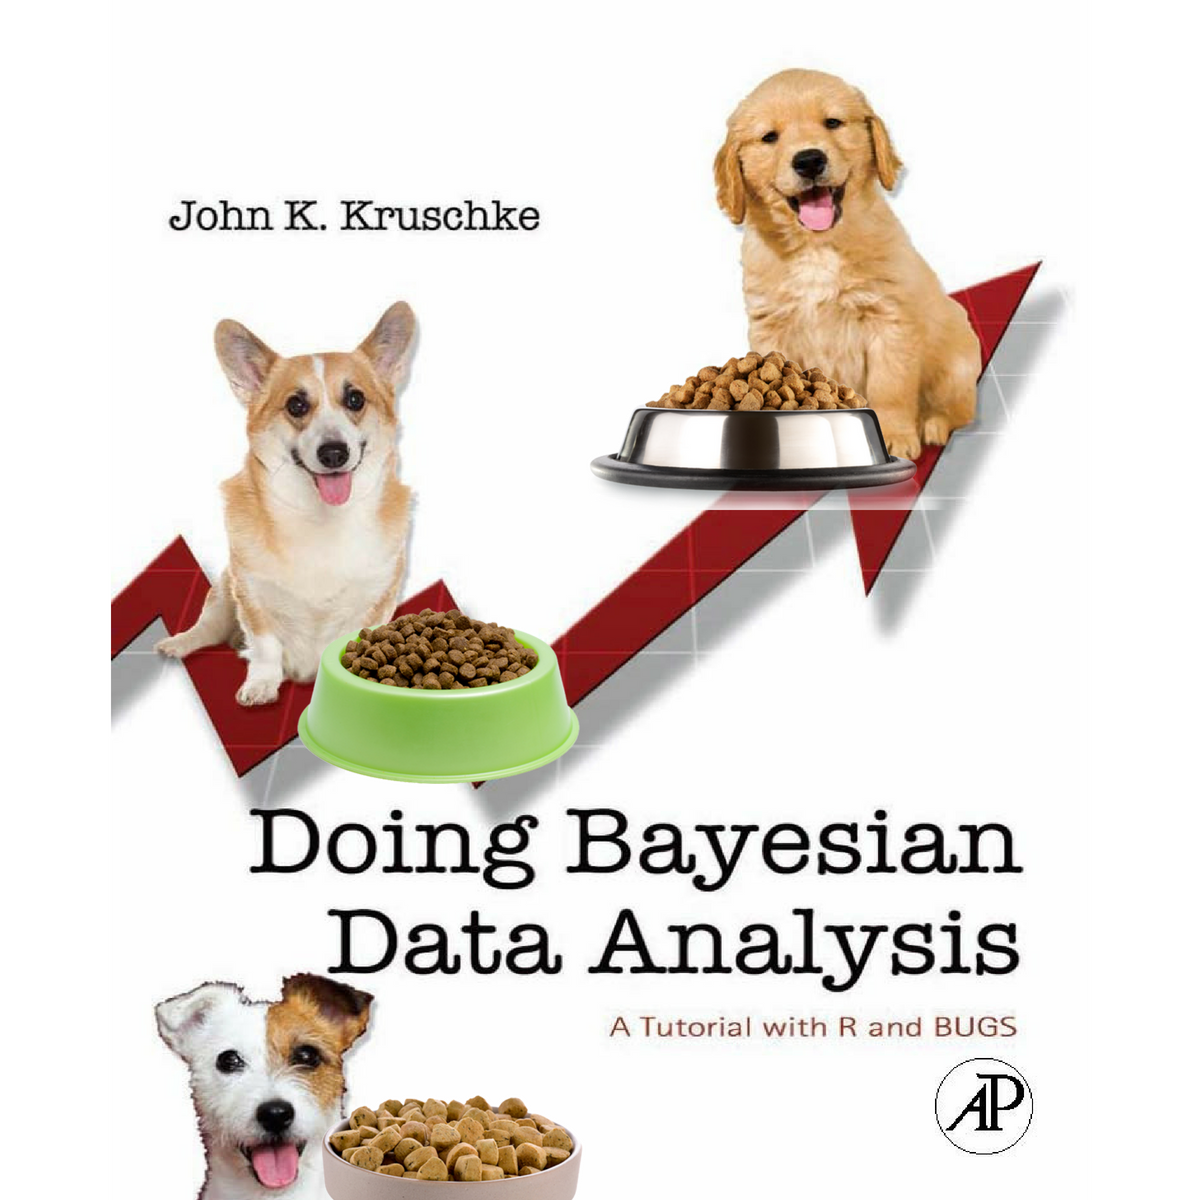
\includegraphics[scale=0.28]{outro.png}
\end{center}
